% !TeX root = ./main.tex
\documentclass[11pt, a4paper, USenglish]{article} % change ``USenglish'' to ``norsk'' if applicable.

\setlength{\marginparwidth}{2cm}
\usepackage{kyblab} % Contains all included packages. See kyblab.sty.
\addbibresource{bibliography.bib} % Makes the bibliography file available to biblatex.

\begin{document}

% Titlepage
\title{Image Processing - Assignment 2}
\author{Group 3\\Martin Eek Gerhardsen}
\date{October 25}
\begin{titlepage}
    \maketitle
    \begin{figure}
    \centering
    
\includegraphics[width=0.5\textwidth]{figures/itk_ntnu}\\
    Department of Engineering Cybernetics
    \end{figure}
    \thispagestyle{empty}
\end{titlepage}

% TOC
\newpage
\tableofcontents
\thispagestyle{empty} % Avoid page numbering on the table of contents.

% Main content
\newpage
\setcounter{page}{1}
\section{Spatial Filtering}

\subsection{Task 1: Theory}
\subsubsection*{a)}
Sampling is the process of converting a continuos-time signal to a discrete-time signal, usually by measuring the continuos-time signal at specific points in time and extending this measurement over a set time step. 

\subsubsection*{b)}
Quantization is the process of constraining a signal from a larger to a smaller set of values, like mapping colours to the standard RGB range of 256 integer values. 

\subsubsection*{c)}
A high contrast image histogram would look similar to a dirac delta function, with most values grouped together around the same intensity.

\subsubsection*{d)}
\begin{table}[]
    \label{tab:initial_image}
    f = \begin{tabular}{|l|l|l|l|l|}
        \hline
        5 & 0 & 2 & 3 & 4 \\ \hline
        3 & 2 & 0 & 5 & 6 \\ \hline
        4 & 6 & 1 & 1 & 4 \\ \hline
    \end{tabular}
\end{table}
\begin{align*}
    n_{\text{pixel}} &= 3 * 5 = 15 \\
    L = 7
    i_0 &= 2 \\ 
    i_1 &= 2 \\
    i_2 &= 2 \\
    i_3 &= 2 \\
    i_4 &= 3 \\
    i_5 &= 2 \\
    i_6 &= 2 \\
    i_7 &= 0
\end{align*}
Then using \cref{eq:equalizer} on \cref{tab:initial_image} gives \cref{tab:equalized_image}. 

\begin{align*}
    \begin{bmatrix}
        n   & 0             & 1             & 2             & 3             & 4             & 5             & 6             & 7 \\ \hline
        f_n &\frac{2}{15} &\frac{2}{15} &\frac{2}{15} &\frac{2}{15} &\frac{3}{15} &\frac{2}{15} &\frac{2}{15} &\frac{0}{15} \\
        F_n &\frac{2}{15} &\frac{4}{15} &\frac{6}{15} &\frac{8}{15} &\frac{11}{15} &\frac{13}{15} &\frac{15}{15} &\frac{15}{15} \\
        E_q & 0 & 1 & 2 & 3 & 4 & 5 & 6 & 6
    \end{bmatrix}
\end{align*}

\begin{equation}
    \label{eq:equalizer}
    g_{i,j} = floor((L - 1) * \sum_{n = 0}^{f_{i,j}} \frac{i_n}{n_{\text{pixel}}}) = floor((L - 1) * F_n)
\end{equation}

\begin{table}[]
    \label{tab:equalized_image}
    \begin{tabular}{|l|l|l|l|l|}
        \hline
        6 & 0 & 2 & 3 & 4 \\ \hline
        3 & 2 & 0 & 5 & 6 \\ \hline
        4 & 6 & 1 & 1 & 4 \\ \hline
    \end{tabular}
\end{table}

\subsubsection*{e)}
The log transform will increase the output intensity for low input intensities, and flatten for high input intensities. This will make it easier to see the lower ranges of the input intensities. If we then apply this transform to 


\newpage
\subsection{Task 2: Programming}
\subsubsection*{a)}
See the result from \cref{fig:greyscale}. 
\begin{figure}[]
    \centering
    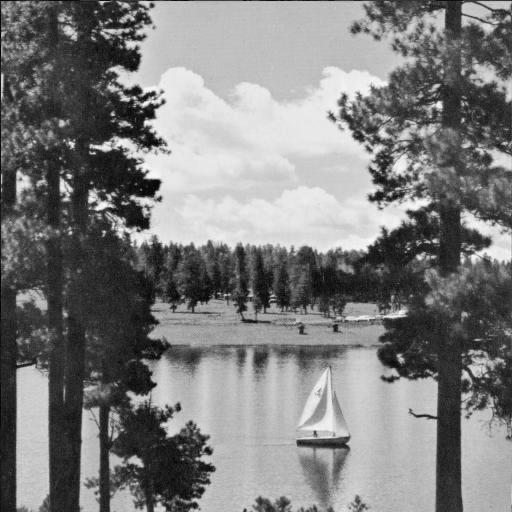
\includegraphics[width=1.00\textwidth]{figures/image_processed/lake_greyscale.jpg}
    \caption{The grey scale version of the lake image}
    \label{fig:greyscale}
\end{figure}

\subsubsection*{b)}
Se the result from \cref{fig:inverse}. 
\begin{figure}[]
    \centering
    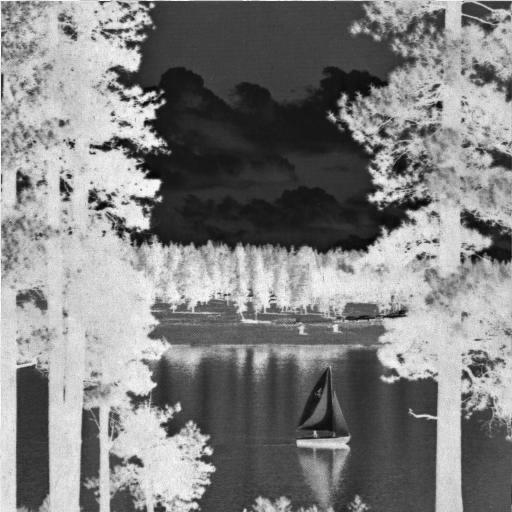
\includegraphics[width=1.00\textwidth]{figures/image_processed/lake_inverse.jpg}
    \caption{The inverse of the grey scale version of the lake image}
    \label{fig:inverse}
\end{figure}

\subsubsection*{c)}
See the results from \cref{fig:convolution_h_a} and \cref{fig:convolution_h_b}.

\begin{figure}[]
    \centering
    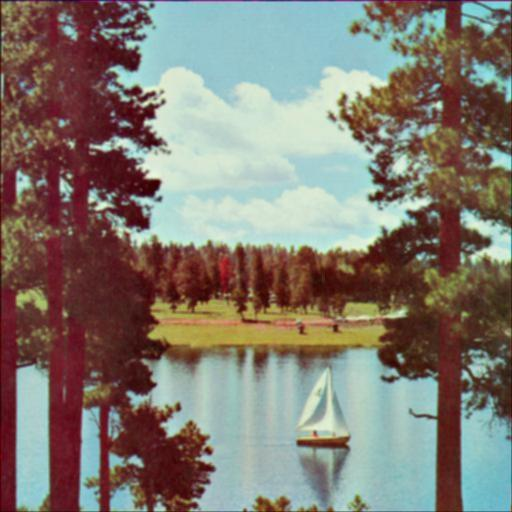
\includegraphics[width=1.00\textwidth]{figures/image_processed/convolved_im_h_a.jpg}
    \caption{Convolution of the lake image with the kernel $h_a$.}
    \label{fig:convolution_h_a}
\end{figure}

\begin{figure}[]
    \centering
    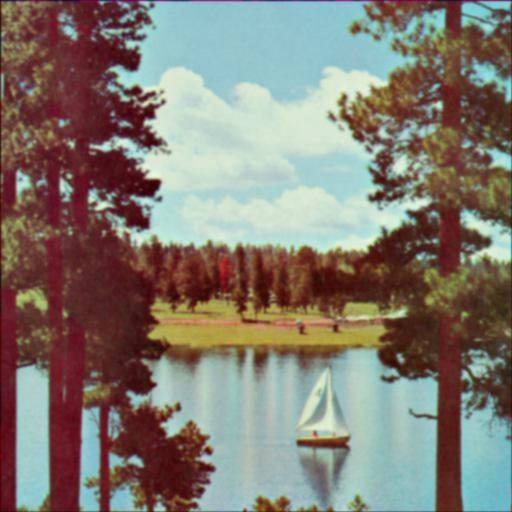
\includegraphics[width=1.00\textwidth]{figures/image_processed/convolved_im_h_b.jpg}
    \caption{Convolution of the lake image with the kernel $h_b$.}
    \label{fig:convolution_h_b}
\end{figure}

\section{Filtering in the Frequency Domain}
\subsection{Task 3: Theory}
\subsubsection*{a)}
From the convolution theorem, we can see that the Fourier transform of a convolution of two signals is multiplication of the Fourier transforms of those individual signals. So a stepwise description would be: 
\begin{itemize}
    \item Find the Fourier transform of the individual signals (i.e. using FFT)
    \item Pointwise multiply the transformed signals
    \item Use inverse Fourier transform to find the convolution of the original signals
\end{itemize}

\subsubsection*{b)}
Low- and high-pass filters tell us which frequencies should be kept, low-pass allows low frequencies to pass, and high-pass allows high frequencies to pass. 

This means that low-pass filters should be close to the filter gain (i.e. 1) frequencies closer to the origin than the cut-off frequency (low frequencies), and should be close to zero for higher frequencies than the cut-off frequency. Depending on how we want the filter to behave, the filter can either be similar to a cylinder or a cone, where cylinder gives a much \textit{harsher} cut-off frequency (no frequencies after cut-off) and cone gives a \textit{smoother} cut-off frequency (allowing, but suppressing some frequencies after cut-off). 

The high-pass filter is simply the $K - LPF$, where $K$ is the filter gain (i.e. 1 again) and $LPF$ is the low-pass filter. This implies that the high-pass filter follows the same pattern as the low-pass, but where the low-pass filter includes frequencies, the high-pass filter removes them, and vice versa where the high-pass includes the frequencies. 

\subsubsection*{c)}
As the images are shifted, we find the low frequencies in the centre and high around the image. Also using the white parts of the images as high amplitude, and black as low amplitude. 

a)
This is primarily a high-pass filter, as the lower frequencies are suppressed. This filter is primarily a high-pass filter along the y-axis (so high frequencies are only allowed given that they are along the y-axis), rather than both x and y. 

b)
This is a high-pass filter, the lower frequencies in the centre are largely suppressed, and the higher frequencies are multiplied with values closer to 1. Though, as the values closest to the x- and y-axes are slightly darker than the diagonals for high frequencies, the filter prefers the signal to have both high frequencies in x and y at the same time. 

c)
This is a low-pass filter, the lower frequencies in the centre are largely included, while the higher frequencies are suppressed.

\newpage
\subsection{Task 4: Programming}
\subsubsection*{a)}
The high-pass filtered image, with the amplitude of the Fourier transforms, can be seen from \cref{fig:camera_high_pass}, and similarly for the low-pass filtered image from \cref{fig:camera_low_pass}. 

\begin{figure}[]
    \centering
    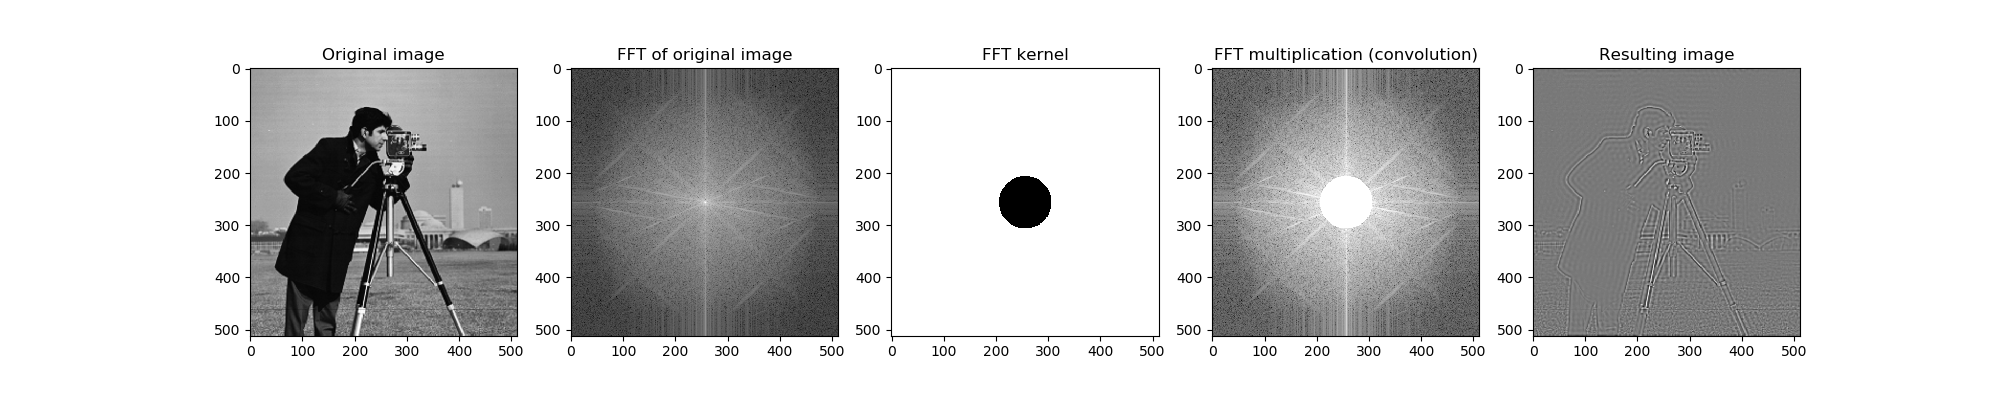
\includegraphics[width=1.00\textwidth]{figures/image_processed/camera_high_pass_subplots.png}
    \caption{High-pass filtered camera man}
    \label{fig:camera_high_pass}
\end{figure}

\begin{figure}[]
    \centering
    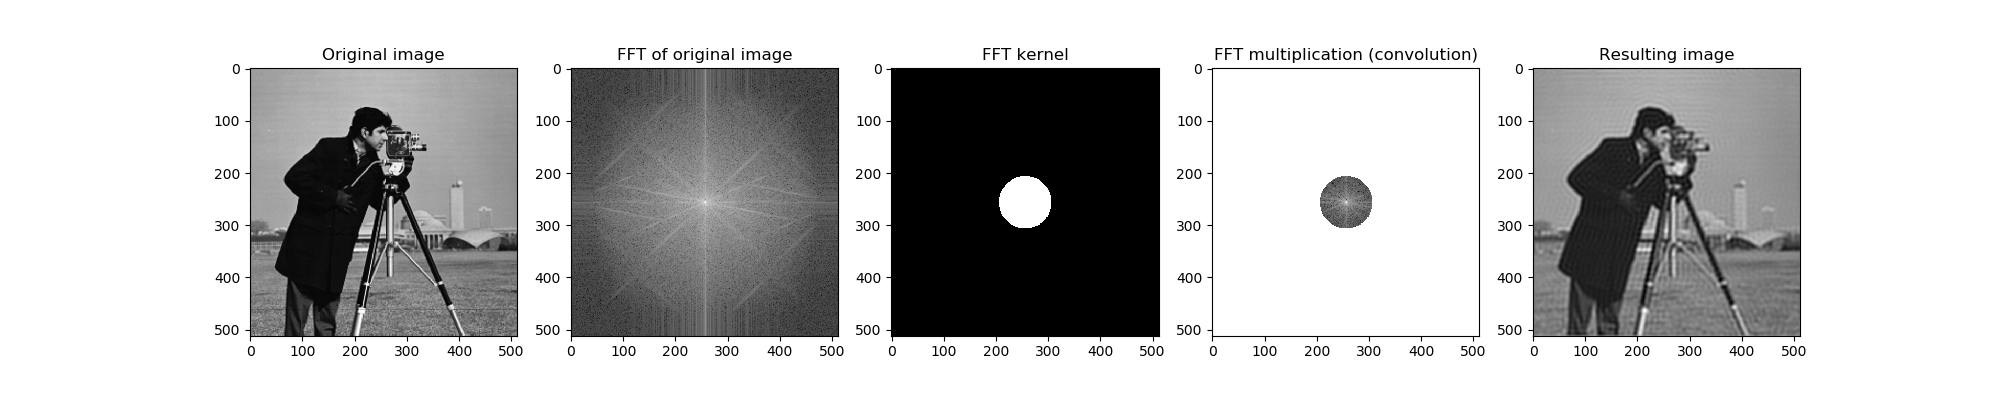
\includegraphics[width=1.00\textwidth]{figures/image_processed/camera_low_pass_subplots.png}
    \caption{Low-pass filtered camera man}
    \label{fig:camera_low_pass}
\end{figure}

\subsubsection*{b)}
The image convolution process for the gaussian kernel can be seen from \cref{fig:camera_gaussian}, and the image convolution process for the horizontal sobel filter can be seen from \cref{fig:camera_sobelx}

\begin{figure}[]
    \centering
    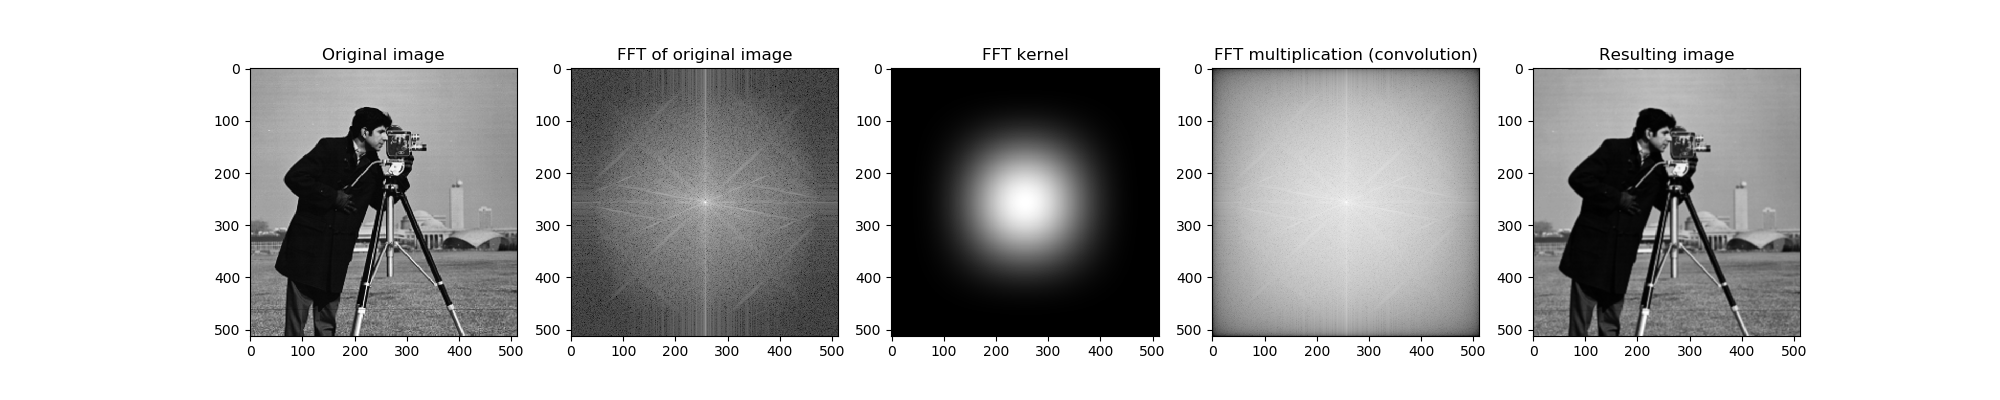
\includegraphics[width=1.00\textwidth]{figures/image_processed/camera_gaussian_subplots.png}
    \caption{Gaussian filtered camera man}
    \label{fig:camera_gaussian}
\end{figure}

\begin{figure}[]
    \centering
    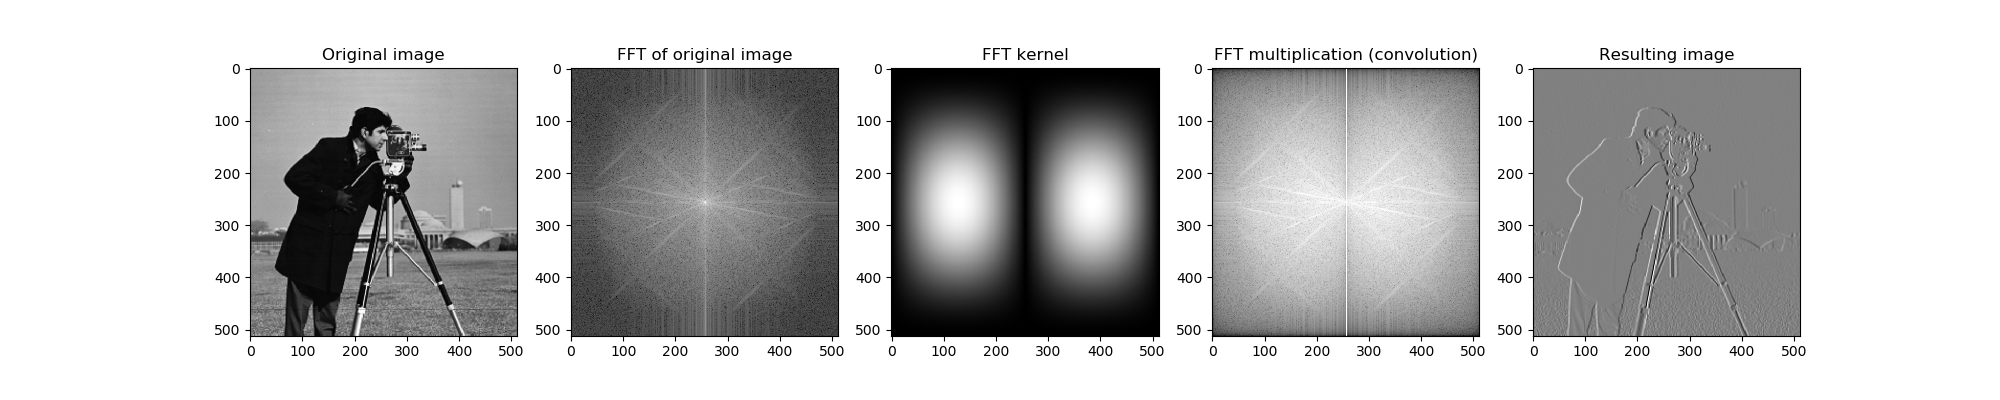
\includegraphics[width=1.00\textwidth]{figures/image_processed/camera_sobelx_subplots.png}
    \caption{Horizontal sobel filtered camera man}
    \label{fig:camera_sobelx}
\end{figure}

\subsubsection*{c)}
The image convolution process for the mystery-filtering can be seen from \cref{fig:clown_filtered}. It is pretty simple to see that this filter removes certain filter-bands, which implies that this is a combination of a four notch filters, or inverse bandpass filters. This then \textit{removes} certain bands of frequencies along the x-axis and y-axis. 

From the Fourier transform of the image, we can see that certain frequencies are very prevalent, and this filter removes those specific points. These were the primary causes for the picture being so wave-y before applying the filter. 

To conclude, I'd call this filter a notch filter (or more accurately a combination of four notch filters). 

\begin{figure}[]
    \centering
    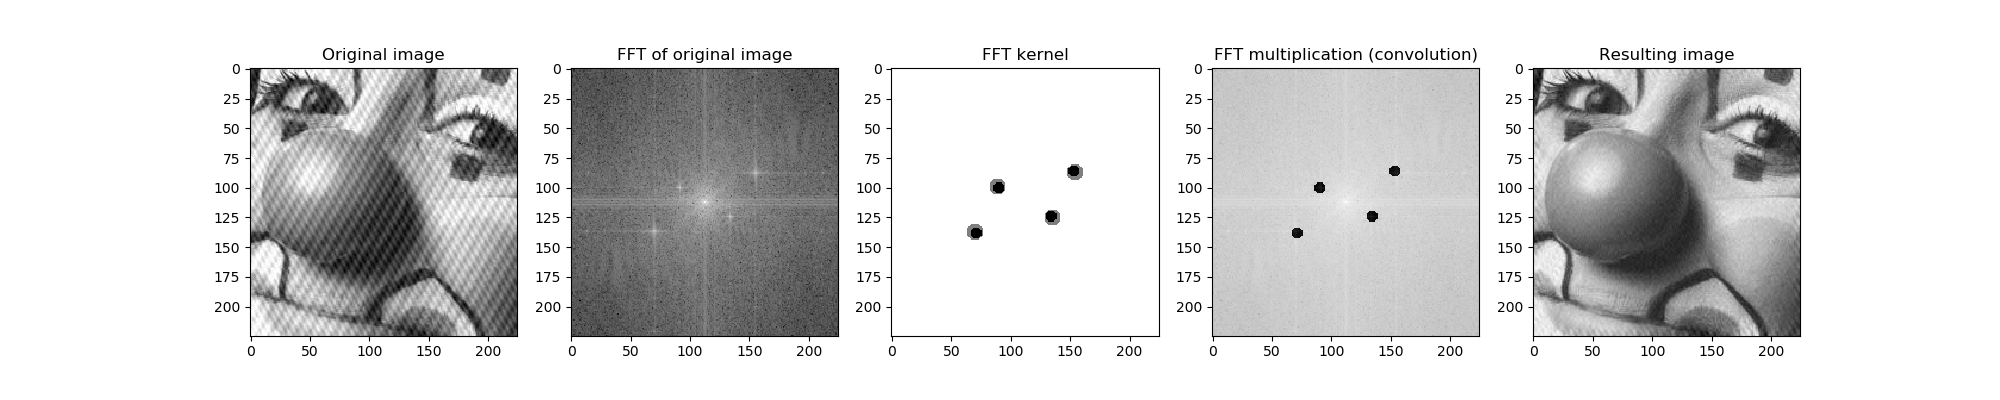
\includegraphics[width=1.00\textwidth]{figures/image_processed/clown_filtered_subplots.png}
    \caption{Mystery-filtered clown (notch filter)}
    \label{fig:clown_filtered}
\end{figure}

\subsubsection*{d)}
See the sharpened image from \cref{fig:moon_sharpened}.

\begin{figure}[]
    \centering
    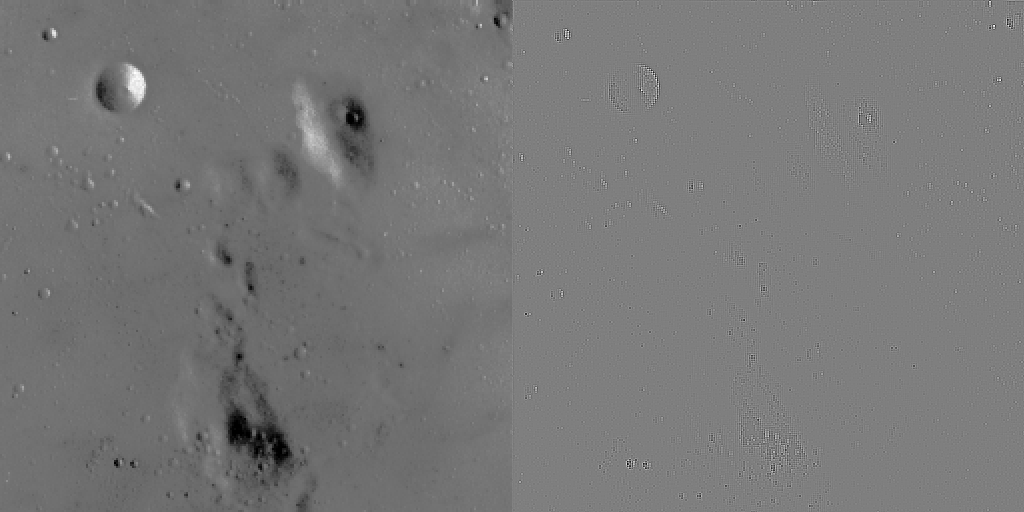
\includegraphics[width=1.00\textwidth]{figures/image_processed/moon_sharpened.png}
    \caption{The original and the sharpened image}
    \label{fig:moon_sharpened}
\end{figure}
% \input simply inserts the contents of the file, while \include forces a \newpage.
% See \input vs. \include: http://tex.stackexchange.com/questions/246/when-should-i-use-input-vs-include

% References
\newpage
\addcontentsline{toc}{section}{References}
% \printbibliography{}
\label{sec:bibliography}

\end{document}
